\begin{figure}[htbp! ]
	\label{pic:6}
	\center{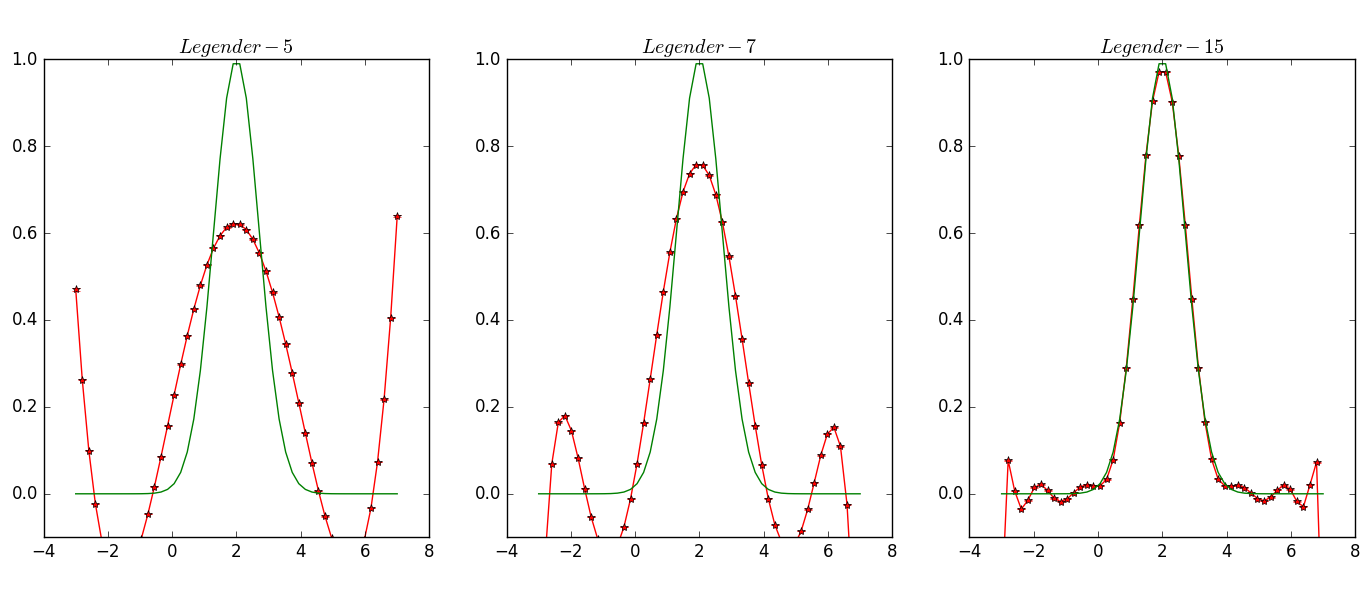
\includegraphics[width=1\linewidth]{pic6} }
	\caption{Восстановление функции Гаусса $e^{-(x-2)^2}$ с помощью 5, 7 и 15 полиномов Лежандра соответственно. Зеленая линия --- исходная функция, красная линия с точками --- результат восстановления.}
\end{figure}

\begin{figure}[htbp! ]
	\label{pic:7}
	\center{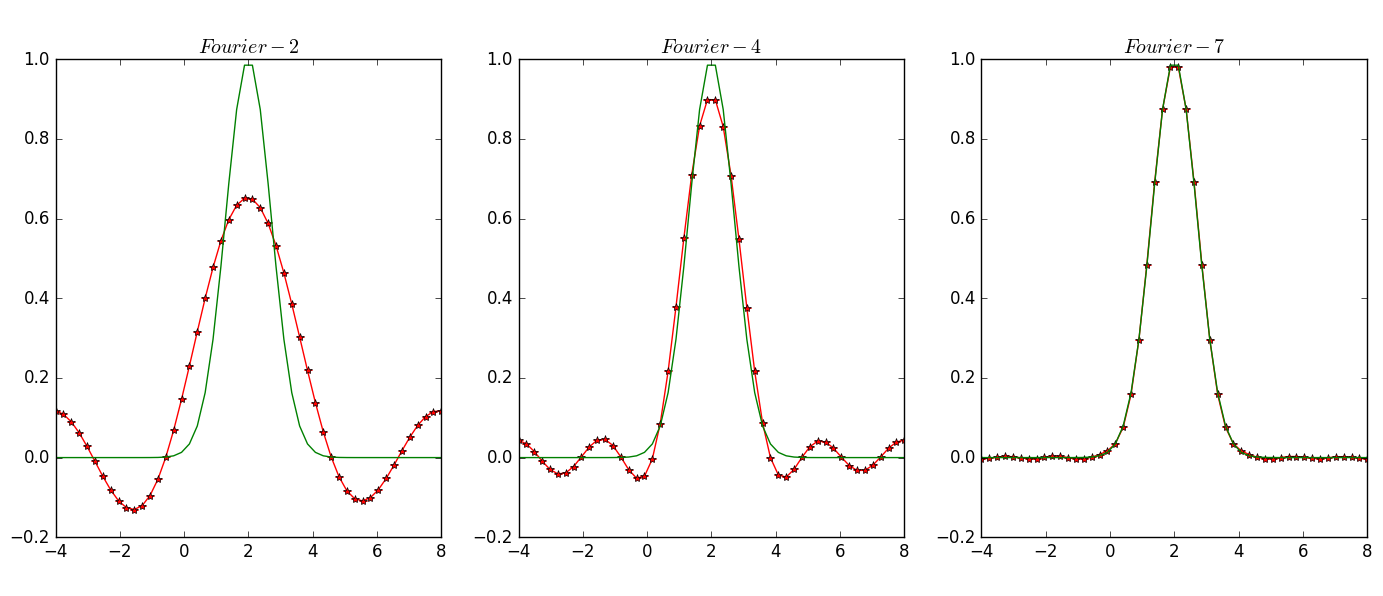
\includegraphics[width=1\linewidth]{pic7}}
	\caption{Восстановление функции Гаусса $e^{-(x-2)^2}$ с помощью 4, 8 и 14 компонент Фурье соответственно. Зеленая линия --- исходная функция, красная линия с точками --- результат восстановления.}
\end{figure}

\begin{figure}[htbp! ]
\begin{center}
\begin{minipage}[h]{0.3\linewidth}
	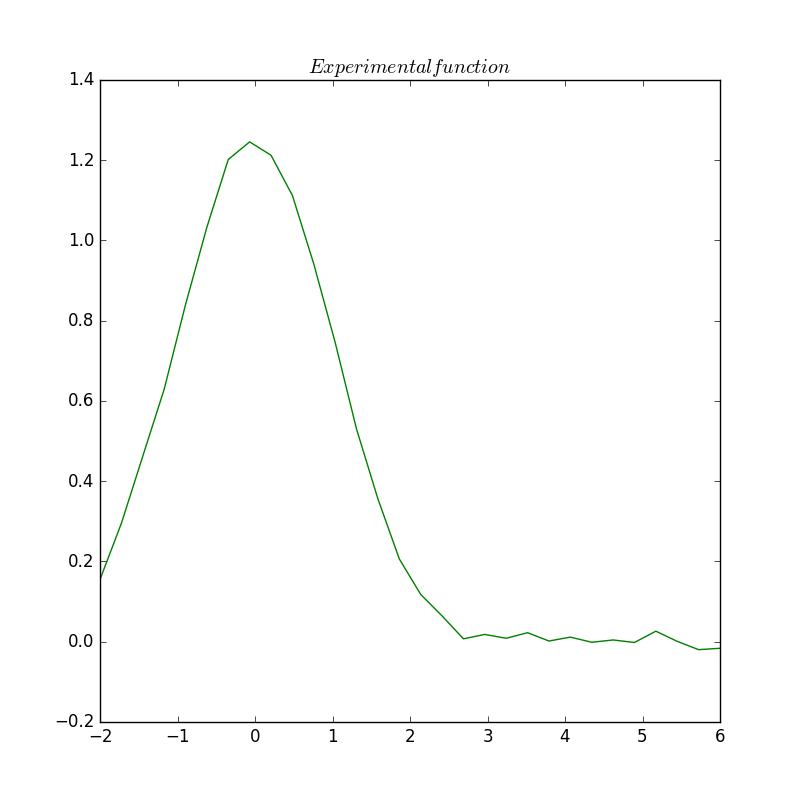
\includegraphics[width=1\linewidth]{func_10} \\а)
\end{minipage}
	\hfill
\begin{minipage}[h]{0.3\linewidth}
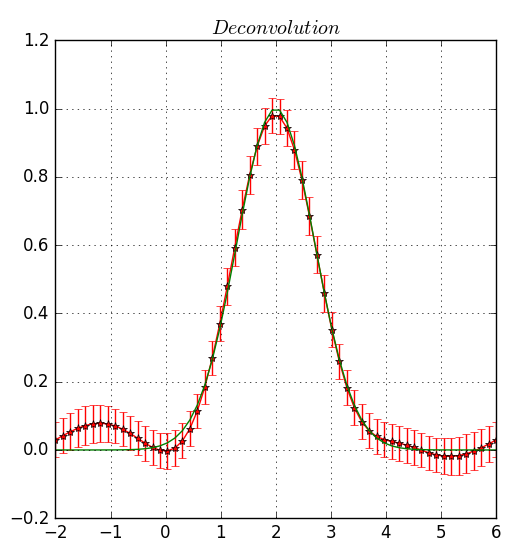
\includegraphics[width=1\linewidth]{pic10a} \\б)
\end{minipage}
\hfill
\begin{minipage}[h]{0.3\linewidth}
	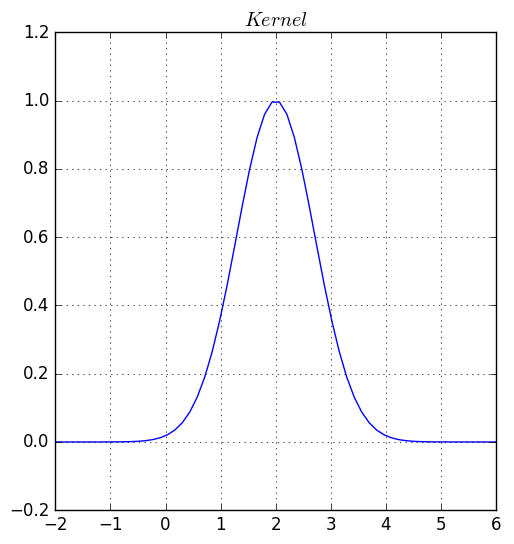
\includegraphics[width=1\linewidth]{pic10b} \\в)
\end{minipage}
	\caption{Случай неинтегрального ядра. а) Экспериментальные значения. б) Ядро $K=e^{-(x-2)^2}$. в) Результат восстановления с помощью базиса Фурье (20 компонент) со статистическими погрешностями 1\%, зеленая линия --- исходная функция, красная линия с точками --- результат регуляризации.}
\label{pic:gausskernel}
\end{center}
\end{figure}

\begin{figure}[htbp! ]
	\center{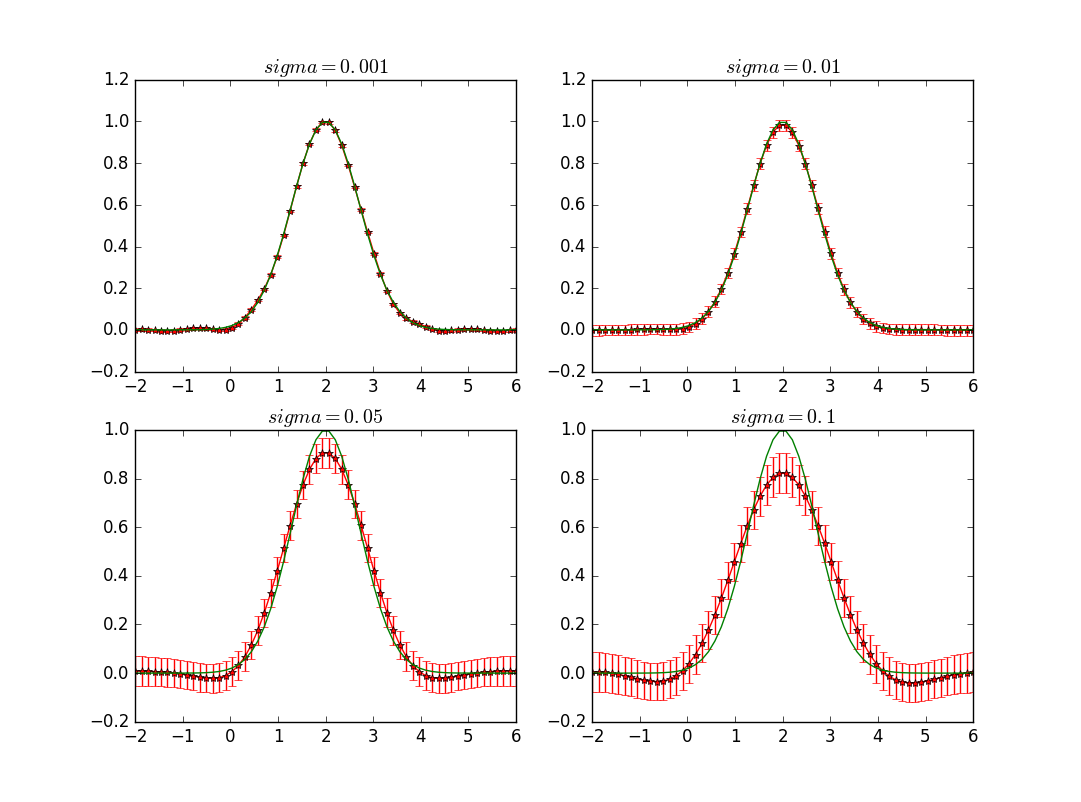
\includegraphics[scale=0.45]{pic12}}
	\caption{Восстановление гаусса с разными погрешностями при измерении: 0.001\%, 1\%, 5\% и 10\%. Зеленая линия --- исходная функция, красная линия с точками --- результат восстановления.}
	\label{pic:noize}
\end{figure}

\begin{figure}[htbp!]
\begin{center}
\begin{minipage}[h]{0.45\linewidth}
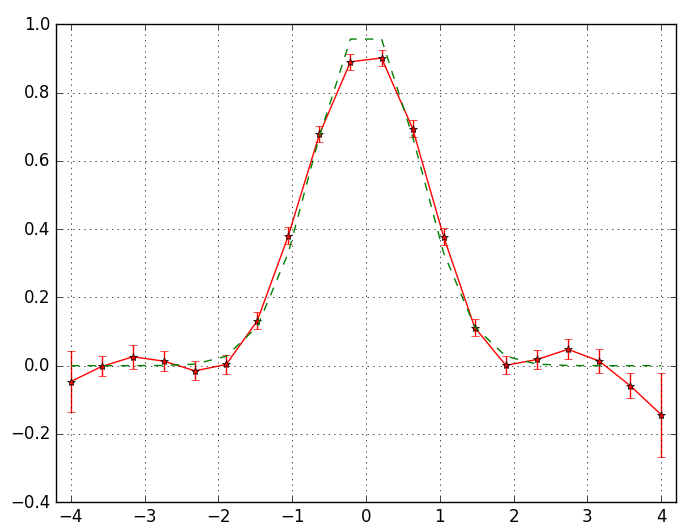
\includegraphics[width=1\linewidth]{no-negative1} \\а)
\end{minipage}
\hfill 
\begin{minipage}[h]{0.45\linewidth}
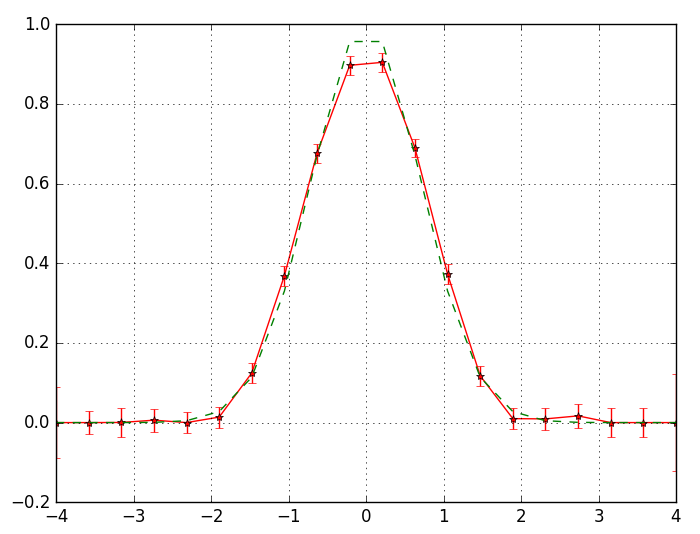
\includegraphics[width=1\linewidth]{no-negative2} \\б)
\end{minipage}
\caption{а) Результат регуляризации до добавления дополнительной информации. б) Результат оптимизации решения. Зеленая линия --- исходная функция, красная линия с точками --- результат регуляризации.}
\label{pic:aprioriopt}
\end{center}
\end{figure}

\begin{figure}[htbp! ]
	\label{pic:exp1}
	\center{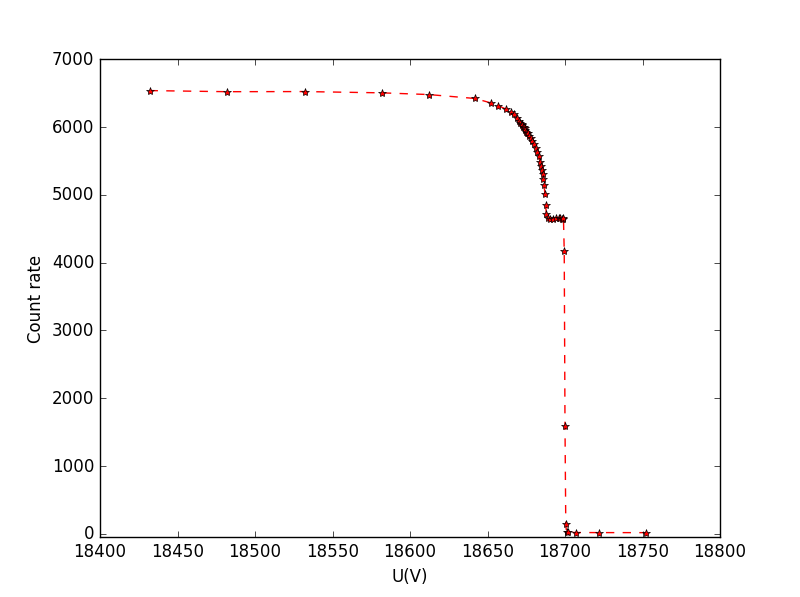
\includegraphics[width=1\linewidth]{exper_data}}
	\caption{Экспериментальные данные --- спектр рассеянных электронов при энергии пушки 18700 eV.}
\end{figure}

\begin{figure}[htbp! ]
	\label{pic:exp3}
	\center{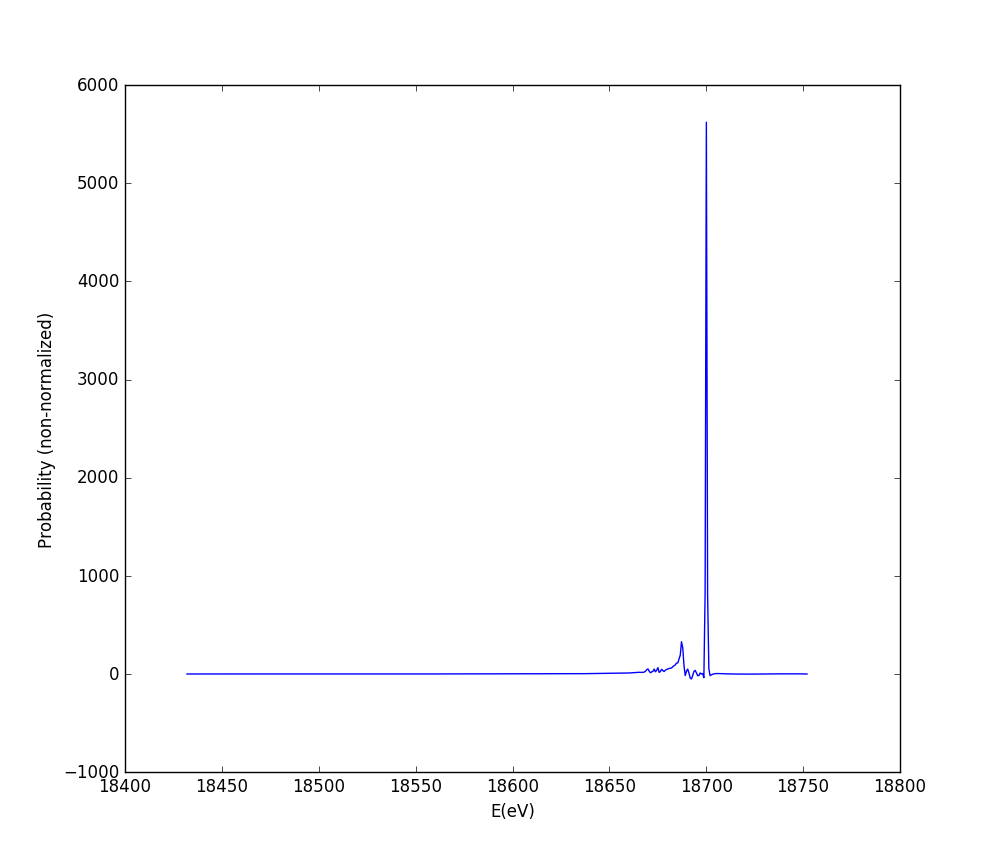
\includegraphics[width=0.75\linewidth]{exp_full}}
	\caption{Результат обработки данных эксперимента Троицк ню-масс.}
\end{figure}

\begin{figure}[htbp! ]
	\label{pic:exp2}
	\center{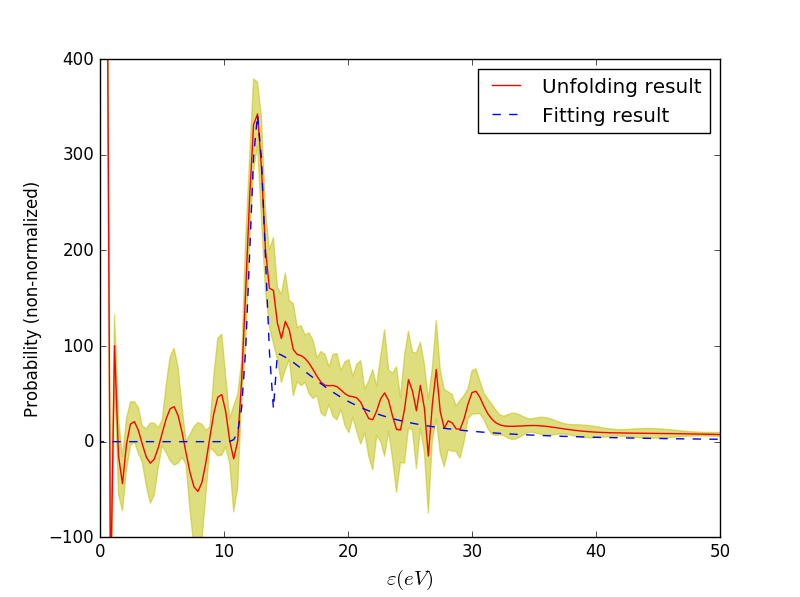
\includegraphics[width=0.75\linewidth]{experim}}
	\caption{Результат обработки данных эксперимента Троицк ню-масс (красная линия) и результат фитирования (пунктирная линия), область одинарного рассеяния.}
\end{figure}